\chapter{DevOps}

In Project-based Software Engineering, there was a \textit{development team} responsible for developing (design, requirements, specification, prototypes, testing, integrating everything, and finally delivering tested software ready for release), and an \textit{operations team} that was responsible for deploying and maintaining the system (by providing user support and possibly making software changes).

The issues with this model were communication delays between teams, separate teams using different tools, having different skills, or often not understanding each other's problems. Additionally, days were required to fix urgent bugs or security vulnerabilities (because the operations team didn't develop the software in the first place).

\noindent Three factors enabled a change:

\begin{itemize}
    \item Agile software engineering \textbf{reduced software development time}, so the traditional release process became a bottleneck.
    \item Amazon re-engineered its software into (micro)services, \textbf{assigning both service development and service support to the same team}.
    \item \textbf{SaaS release of software} became possible on public/private clouds.
\end{itemize}

\noindent \textbf{DevOps} (\textbf{Dev}elopment + \textbf{Op}eration\textbf{s}) integrates development, deployment, and support into a single team. The DevOps \textbf{principles} are:     
\begin{itemize}
    \item \textbf{Everyone is responsible for everything}: all team members share responsibility for developing, delivering, and supporting the software.
    \item \textbf{Everything that can be automated should be automated}: All/most activities involved in testing, deployment, and support should be automated.
    \item \textbf{Measure first, change later}: DevOps should be driven by measuring collected data about the system and its operation.
\end{itemize}

\newpage
\noindent Some of DevOps' \textbf{benefits} are:

\begin{itemize}
    \item \textbf{Faster deployment} (the main benefit): a dramatic reduction in human communication delays leads to faster deployment to production (from days/weeks to hours).
    \item \textbf{Reduced risk}: small functionality increments in each release reduce the chance of feature interactions and system failures/outages.
    \item \textbf{Faster repair}: no need to discover which team is responsible for fixing a problem and wait for them to resolve it.
    \item \textbf{More productive teams}: DevOps teams are more productive than teams involved in separate activities.
\end{itemize}

Creating a \textbf{DevOps team} means bringing together a variety of skill sets, including software engineering, UX design, security engineering, infrastructure engineering, customer interaction, and more. The success of a DevOps team is based on a \textbf{culture of mutual respect and sharing} (everyone on the team should be involved in Scrums and other team meetings, and team members are encouraged to share their expertise with others and learn new skills) and the \textbf{support from developers for the software they have developed} (if a service fails on the weekend, the developer is responsible for getting it up and running again. If a developer is unavailable, other team members take over the task. DevOps teams focus on fixing failures as quickly as possible rather than blaming team member(s)).

\section{Code management}

During the development of a software product, tens of thousands of lines of code are written, and automated tests are created, organized into hundreds of files. Dozens of libraries are used, and different programs are needed to create/run the code, making it impossible to keep track of changes made to the software without automated support.

A \textbf{code management system} is software that supports practices to manage an evolving codebase. It is important that the \textit{code management system} ensures that changes made by different developers do not interfere with each other and that it helps create different product versions. A \textit{code management system} should also simplify the creation of an executable product from source code files and the running of automated tests. Figure \ref{fig:code-management-system} shows the components of a code management system: at the top, there's the CI/CD\footnote{CI/CD: Continuous Integration/Continuous Deployment-Delivery} pipeline, at the bottom, the DevOps measurement, and in the middle, the code management system. Inside the middle box, the main functionalities of a code management system are listed.

\begin{figure} [H]
    \centering
    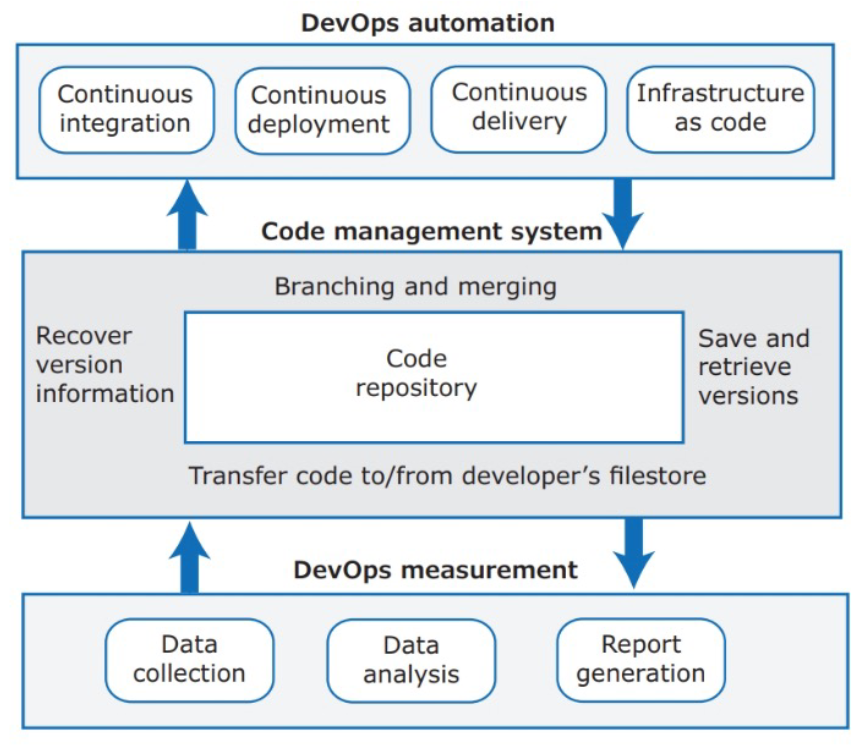
\includegraphics[width=0.75\textwidth]{images/DevOps/code-management-system.png}
    \caption{DevOps system structure}
    \label{fig:code-management-system}
\end{figure} 

\noindent \textbf{Features} of code management systems are:
\begin{itemize}
    \item \textbf{Version and release identification}: managed versions of a code file are uniquely identified when submitted to the system (managed files can never be overwritten). They can be retrieved using their identifier and other file attributes.
    \item \textbf{Change history recording}: when a change to a code file is submitted, the submitter must add a note explaining the reasons for the change. This helps developers understand why a new version was created.
    \item \textbf{Independent development}: several developers can work on the same code file simultaneously. When submitted to the code management system, a new version is created, ensuring files are never overwritten by later changes, avoiding the file overwriting problem.
    \item \textbf{Project support}: developers download code into a personal file store, work on it, and return it to the shared code management system. Parallel development branches can be created for concurrent work, and changes made in different branches may be merged. All files associated with a project may be checked out simultaneously.
    \item \textbf{Storage management}: the code management system includes efficient storage mechanisms to avoid keeping multiple copies of files with only small differences (less critical today with cheaper storage).
\end{itemize}

Initially, centralized systems were used for project support, but the \textbf{advantages of decentralized systems} (e.g., Git (\textit{Linux’s Distributed Version Control System})) have made decentralized systems the best solution. These advantages include:

\begin{itemize}
    \item \textbf{Resilience}: Everyone working on a project has their own copy of the repository (and people can work offline as well). If the shared repository is damaged or attacked, work can continue, and clones can be used to restore the shared repository.
    \item \textbf{Speed}: committing changes to the repository is a fast operation since commits can be made both locally (without the need for data transfer over the network) and in the general branch.
    \item \textbf{Flexibility}: since everyone has their own copy, local experimentation is much simpler and safer.
\end{itemize}

A famous decentralized system is \textbf{Git}, where there are both \textit{private clones} of the shared repository on each developer’s computer and a \textit{shared project} repository (running on the company’s server or in the cloud hosted by services like GitHub or GitLab). Figure \ref{fig:git} shows some \textit{Git commands} and what the \textit{Git branch} looks like.

\begin{figure} [H]
    \centering
    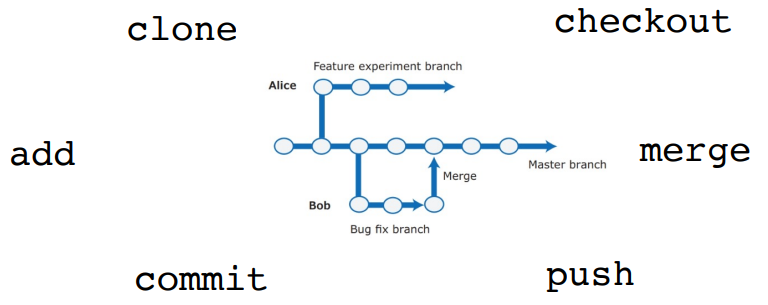
\includegraphics[width=1\textwidth]{images/DevOps/git.PNG}
    \caption{Git branch example}
    \label{fig:git}
\end{figure} 

When discussing \textit{Open-source software development} with Git, there's usually a group of people who decide what changes should be incorporated. GitHub uses a mechanism called \textit{Webhooks} to trigger DevOps automation tools in response to updates to the project repository.

\newpage

\section{DevOps automation}

\textbf{Everything that can be should be automated}. This was one of the DevOps principles that we'll discuss in detail in this section of the chapter. The following section will be divided into:
\begin{itemize}
    \item \textbf{Continuous integration}: Each time a developer commits a change to the project’s master branch, an executable version of the system is built and tested.
    \item \textbf{Continuous delivery}: Once the new version is built, executable software is tested in a simulated product’s operating environment.
    \item \textbf{Continuous deployment}: A new release of the system is made available to users every time a change is made to the master branch of the software.
    \item \textbf{Infrastructure as code}: Machine-readable models of infrastructure (network, servers, routers, etc.) on which the product executes are used by configuration management tools to build the software’s execution platform. The software to be installed, such as compilers, libraries, and a DBMS, are included in the infrastructure model.
\end{itemize}

\subsection{Continuous integration}

The reason why continuous integration should be used is that if a system is infrequently integrated, \textbf{problems can be difficult to isolate}, and fixing them slows down system development. System integration (\textit{system building}) is more than compiling:
\begin{enumerate}
    \item Install database software and set up the database with the appropriate schema.
    \item Load test data into the database.
    \item Link compiled code with libraries and other components used.
    \item Check that external services used are operational.
    \item Move configuration files to the correct locations (and delete old ones).
    \item Run system tests to check that integration has been successful.
\end{enumerate}

As we can see from Figure \ref{fig:continuous-integration}, an integrated version of the system is created and tested every time a change is pushed to the system’s shared code repository. On completion of the push operation, the repository sends a message to the integration server to build a new version of the product.

\begin{figure} [H]
    \centering
    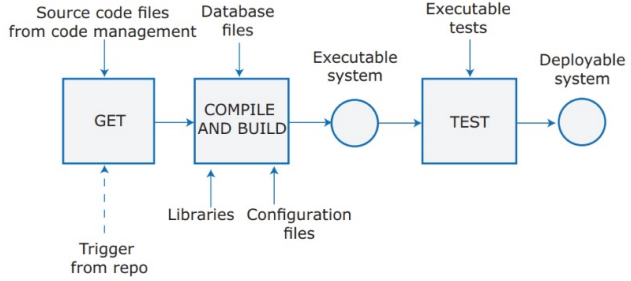
\includegraphics[width=0.8\textwidth]{images/DevOps/continuos-integration.PNG}
    \caption{Continuous integration pipeline}
    \label{fig:continuous-integration}
\end{figure} 

It's good practice to adopt an \textbf{integrate twice} approach to system integration, which consists of a first integration on the local developer machine, and then a second one where the code is pushed to the project repository to trigger the integration server (as we can see from Figure \ref{fig:continuous-integration}). This is done because it is really bad to integrate a broken build into the project repository.

\begin{figure} [H]
    \centering
    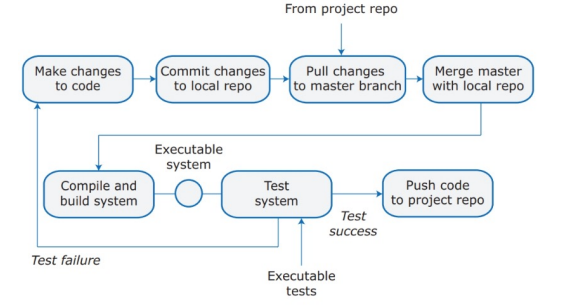
\includegraphics[width=0.8\textwidth]{images/DevOps/integrate-twice.PNG}
    \caption{Integrate twice pipeline}
    \label{fig:continuous-integration}
\end{figure} 

The \textbf{advantages} of continuous integration are:

\begin{itemize}
    \item \textbf{It is faster to find and fix bugs in the system}, since if you make a small change and some system test fails, the problem almost certainly lies in the new code that you pushed.
    \item \textbf{A working system is always available to the whole team}, so it can be used to test ideas and to demo the system to management and customers.
    \item \textbf{“Quality culture” in the development team}, because no team member wants the stigma of breaking the build: everybody checks their work carefully before pushing it to the project repository.
\end{itemize}

Analyzing the whole codebase every time a commit is made is really heavy, which is why \textbf{code integration tools} only repeat actions if dependent files have been changed (e.g., create new object codes only for those whose source code has changed). Modification timestamps can be used to check if some dependencies have changed.

\subsection{Continuous delivery and deployment}

With \textit{Continuous Integration} and \textit{source code management}, it is possible to create an executable version of a software system by building the system and running tests first on the developers' computer and then on the project integration server.

When deploying the executable version of the software into a real production environment, it's possible that something goes wrong since the \textbf{real production environment will differ from the development environment} (because the production server may have a different file system organization, access permissions, installed applications, and so on).

\textbf{Continuous delivery} ensures that the changed system is ready for delivery to customers by performing \textbf{feature tests} in the production environment (to make sure that the environment does not cause system failures), \textbf{system tests}, and \textbf{load tests} (to check how the software behaves as the number of users increases). \textit{Containers} are the simplest way to create a replica of a production environment.

As we can see from Figure \ref{fig:CDCD}, to \textbf{deliver} the new system, a staged test environment is configured (after some initial \textit{integration testing}), and then system acceptance tests (\textit{functionality}, \textit{load}, \textit{performance}) are launched. To \textbf{deploy} it, software and data are transferred to production servers, then a switch to the new system version is made, and finalized with a restart of the process (it's critical to also manage situations where clients are still connected to the old version of the system).

\begin{figure} [H]
    \centering
    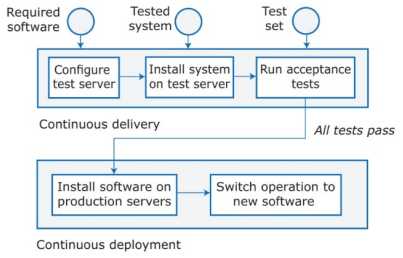
\includegraphics[width=0.6\textwidth]{images/DevOps/CDCD.PNG}
    \caption{Continuous delivery and continuous deployment schema}
    \label{fig:CDCD}
\end{figure} 

\newpage
The \textbf{benefits} of continuous deployment are:

\begin{itemize}
    \item \textbf{Reduced costs}: fully automated deployment pipeline.
    \item \textbf{Faster problem solving}: if a problem occurs, it will probably affect only a small part of the system, and the source of that problem will be obvious.
    \item \textbf{Faster customer feedback}: it is possible to deploy new features when they are ready for customer use, and then users’ feedback can be used to identify improvements.
    \item \textbf{A/B testing}: if there are many customers and several servers, it's possible to deploy a new software version only on some servers and use a load balancer to divert some customers to the new version, in order to measure and assess how new features are used.
\end{itemize}

Notice that it's probably best to \textbf{not deploy every single change}, since small changes may have incomplete features that could be deployed, and it's important to not disclose this to competitors until implementation is complete. Another reason is that customers may be irritated by continually changing software, especially if this affects the UI. Developers may also want to synchronize releases with known business cycles (e.g., the start of the academic year for the education market).

There are many Continuous Integration \textbf{tools} (such as \textit{Jenkins} and \textit{Travis}) that may also be used to support Continuous Delivery and Deployment. These tools can integrate with infrastructure configuration management tools to implement software deployment, even though for \textit{cloud-based software}, it is often simpler to use containers in conjunction with CI tools rather than infrastructure configuration management software.

\subsection{Infrastructure as code}

Manually maintaining a computing infrastructure with tens or hundreds of servers is \textbf{expensive} and \textbf{error-prone}. This is because many different physical/virtual servers have different configurations and run different software packages, so when new versions of software become available, some servers may have to be updated, while others may not, due to dependencies with older versions of software. Tracking manually the software installed on each server is really hard, and not done every time (e.g., emergency changes are not always documented).

It would be nice to automate the process of updating software on servers by using a machine-readable model of the infrastructure: \textbf{Configuration Management} (CM) \textbf{tools} (like \textit{Puppet}, \textit{Chef}, and \textit{Ansible}) can automatically install software and services on servers according to the infrastructure definition (infrastructure is represented as data, that's why we call it IaC (Figure \ref{fig:IaC})). When changes have to be made, the infrastructure definition model is updated, and the CM tool makes the changes to all servers.

\newpage

\begin{figure} [H]
    \centering
    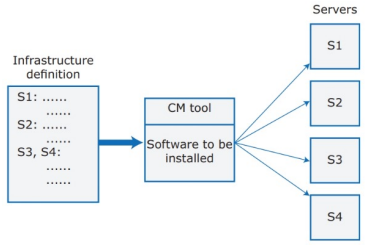
\includegraphics[width=0.6\textwidth]{images/DevOps/IaC.PNG}
    \caption{Infrastructure as code schema}
    \label{fig:IaC}
\end{figure} 

\noindent The \textbf{advantages} of infrastructure as code are:
\begin{itemize}
    \item \textbf{Visibility}: Infrastructure is defined as a stand-alone model that can be read, understood, and reviewed by the whole DevOps team.
    \item \textbf{Reproducibility}: Installation tasks will always be performed in the same sequence, and the same environment will always be created. You do not have to rely on people remembering the order in which they need to do things (computers are superior to humans in terms of reproducibility).
    \item \textbf{Reliability}: Automation avoids simple mistakes made by system administrators when making the same changes to several servers.
    \item \textbf{Recovery}: The infrastructure model can be versioned and stored in a code management system. If infrastructure changes cause problems, you can easily revert to an older version and reinstall the environment that developers know works.
\end{itemize}

\textbf{Containers} are a very effective way to deploy cloud-based products. With containers, it's simple to provide \textbf{identical execution environments} (for each type of server developers use, they define the environment they need and build an image for execution. When developers update the software, they create a new image that includes the modified software). Developers can employ a \textit{container management system} (such as Kubernetes) for scaling, resiliency, and other orchestration properties.

\newpage

\section{DevOps measurement}

In order to continuously \textbf{improve your DevOps process} to achieve faster deployment of better-quality software, measuring and analyzing product and process data is needed.

\noindent There are various types of data measurements:
\begin{itemize}
    \item \textbf{Process measurements}: Collect and analyze data on development, testing, and deployment processes.
    \item \textbf{Service measurements}: Collect and analyze data on software’s performance, reliability, and acceptability to customers.
    \item \textbf{Usage measurements}: Collect and analyze data on how customers use your product instead of using pop-ups that ask if they liked a certain product (this helps to identify issues and problems with the software itself).
    \item \textbf{Business success measurements}: Collect and analyze data on how your product contributes to overall business success (it's hard to isolate the contribution of DevOps to business success since that may be due to DevOps introduction or to better management).
\end{itemize}

Measuring software and its development is a \textbf{complex process}, since developers need to identify suitable metrics that give useful insights and find reliable ways of collecting and analyzing metric data. Some of the measures (e.g., customer satisfaction) must be inferred from other metrics (e.g., the number of returning customers).

Software measurement should be automated as far as possible, so developers must instrument their software to collect data about itself and use a monitoring system to collect data about software’s performance and availability. \newline \noindent In order to collect data automatically, it's possible to:

\begin{itemize}
    \item Use \textbf{continuous integration tools} like Jenkins to collect data on deployments, successful tests, and so on.
    \item Use \textbf{monitoring services} provided by cloud providers like Amazon’s Cloudwatch to collect data on availability and performance.
    \item Collect customer-supplied data from \textbf{issue management systems}.
    \item \textbf{Add instrumentation to a product} to gather data on its performance and how it is used by customers (usually log files are the best option: log as many events as possible, and use log analysis tools to extract useful information on how your software is used).
\end{itemize}

